\documentclass{article}
\usepackage[utf8]{inputenc}  
\usepackage[T1]{fontenc}     
\usepackage{tikz}
\usetikzlibrary{shapes,positioning,arrows,calc}

\begin{document}

% pile : exemple

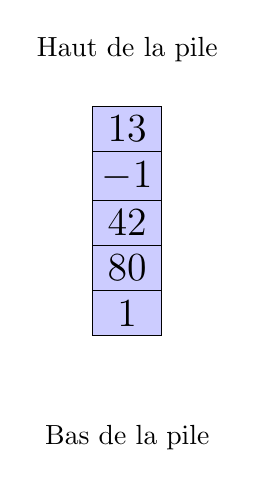
\begin{tikzpicture}[stack/.style={fill=blue!20, font=\sffamily\Large\bfseries, rectangle split, rectangle split parts=5, draw, anchor=center}]

\node [stack] (stack)  {$13$\nodepart{two}$-1$%
   \nodepart{three}$42$\nodepart{four}$80$\nodepart{five}$1$};
\node [above=of stack,anchor=north,align=left] {Haut de la pile};
\node [below=of stack,anchor=north,align=left] {Bas de la pile};

\end{tikzpicture}

% pile : exemple ajout

\vspace{3cm}
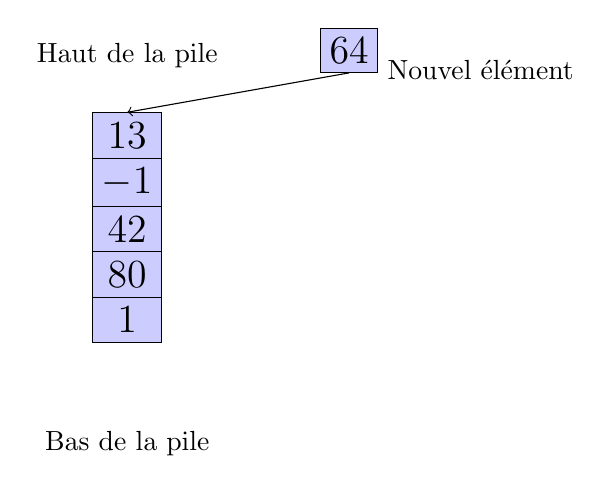
\begin{tikzpicture}[stack/.style={fill=blue!20, font=\sffamily\Large\bfseries, rectangle split, rectangle split parts=5, draw, anchor=center}, new/.style={fill=blue!20, font=\sffamily\Large\bfseries, rectangle, draw, anchor=center}]

\node [stack] (stack)  {$13$\nodepart{two}$-1$%
   \nodepart{three}$42$\nodepart{four}$80$\nodepart{five}$1$};
\node [above=of stack,anchor=north,align=left] {Haut de la pile};
\node [below=of stack,anchor=north,align=left] {Bas de la pile};

\node [new,above right=0.5cm and 2cm of stack] (n) {$64$};
\node [right=1.3cm of n,anchor=north,align=left] {Nouvel élément};
\draw [->] (n.south)--(stack.north);

\end{tikzpicture}


% pile : exemple suppression

\vspace{3cm}
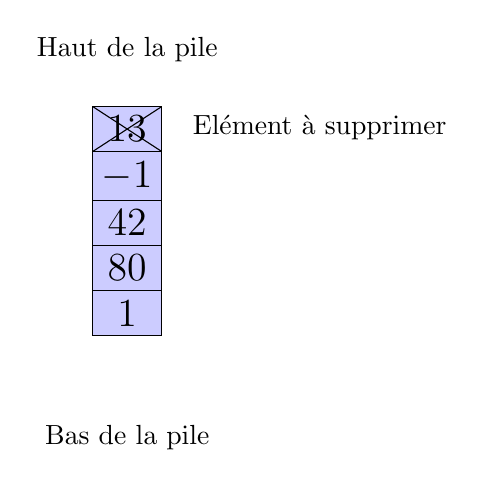
\begin{tikzpicture}[stack/.style={fill=blue!20, font=\sffamily\Large\bfseries, rectangle split, rectangle split parts=5, draw, anchor=center}]

\node [stack] (stack)  {$13$\nodepart{two}$-1$%
   \nodepart{three}$42$\nodepart{four}$80$\nodepart{five}$1$};
\node [above=of stack,anchor=north,align=left] {Haut de la pile};
\node [below=of stack,anchor=north,align=left] {Bas de la pile};
\node [above right=0cm and 2cm of stack,anchor=north,align=left] {Elément à supprimer};
\draw (0.43,1.45) -- (-0.43,0.89);
\draw (0.43,0.89) -- (-0.43,1.45);

\end{tikzpicture}



\end{document}